\documentclass[../main.tex]{subfiles}

\begin{document}
A tsunami is a single or series of ocean waves which are generated by sudden displacements in the sea floor, landslides, or volcanic activity \cite{zirker}. These potentially catastrophic ocean waves frequently occur in a basin of the Pacfic Ocean known as the "Ring of Fire" for its historically intense volcanic activity \cite{zirker}. Further background into the geological mechanisms resposible for tsunamis can be found in Zirker's (2013) introductory text \textit{The Science of Ocean Waves: Ripples, Tsunamis, and Stormy Seas} \cite{zirker}. An example of tsunami generation can be seen in figure~\ref{fig:tsu_gen}, which was taken from chapter 3 of Marghany's (2018) \textit{Advanced Geoscience Remote Sensing} \cite{marghany}. 

\begin{figure}[h]
    \centering
    \fbox{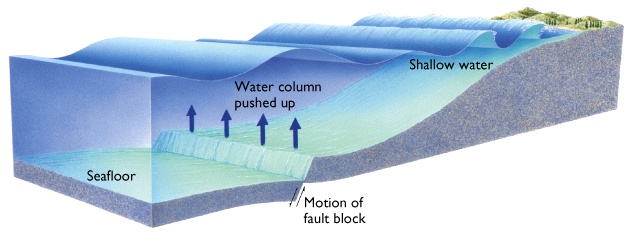
\includegraphics[width=0.75\textwidth]{tsunami_generation}}
    \caption{Tsnumai generation due to horizontal seafloor displacement \cite{marghany}.}
    \label{fig:tsu_gen}
\end{figure}

Transient horizontal displacements resulting from submarine earthquakes and their role in tsunami generation were the focus of  Tanioka' and Satake's (1996) study \textit{Tsunami generation by horizontal displacement of ocean bottom} published in Geophysical Research Letters \cite{satake1}. In this study, they utilize the Satake's (1995) earlier work \textit{Linear and nonlinear computations of the 1992 Nicaragua earthquake tsunami}, which compared and contrasted the success of linear and nonlinear models that governed the generation and propagaion of tsunamis. The linear model utilized in Satake's case study of the Nicaragua earthquake, known as the \textit{shallow-water equations}, and its numerical simulation via a finite-difference method will be the focus of this project.

\end{document}
